	%--------------------------------------------------- Dimension commerciale ------------------------------------------------%

	\part{Dimension commerciale}
	
	\setcounter{chapter}{1} % Pour recommencer la numérotation des chapitres à 1
	\setcounter{section}{0} % Pour recommencer la numérotation des section à 1
	
	\section{Introduction}
	Le projet transversal est issu de la collaboration de l'école polytechnique de l'université de Nantes et de l'entreprise Project2Cloud. Il sera mené de bout en bout par deux étudiants de quatrième année du cycle ingénieur, supervisés par deux professeurs référents. Il s'étendra de septembre à mai. L'objectif est de permettre aux étudiants en charge de réaliser un projet professionnel dans le cadre de leurs études. Au delà de la dimension technique, les projets informatiques intègres des notions plus larges et plus actuelles. Il est donc important de prendre conscience que les projets transversaux présentent des enjeux marketing et écologiques. Il conviendra donc de mettre en œuvre une démarche organisationnelle, qui s'appuiera sur les enseignements dispensés dans les modules Homme Entreprise Société. 
	Nous commencerons par présenter l'entreprise, puis nous détaillerons le projet qui nous a été proposé. Nous terminerons par la problématique marketing que nous avons décidé de développer. 

	\section{L'entreprise : Project2Cloud}
	Project2Cloud est une plate-forme de gestion collaborative. Une site de présentation est déjà en ligne à l'adresse http://project2cloud.org/. Elle propose différents services de communication, tels que la vidéo-conférence, le chat et la conversation audio. Le but est d'offrir aux utilisateurs un panel complet de communication, leur permettant d'échanger en temps réel des informations et des services. Project2Cloud innove également avec la possibilité d'associer aux sessions de dialogue des documents de différents types (texte, vidéos...). Le document associé à la session permet de créer une "mémoire" numérique du document, autour de laquelle de nouvelles connaissances peuvent venir s'ajouter à tout moment. 

			\begin{figure}[H] 
				\begin{center}
					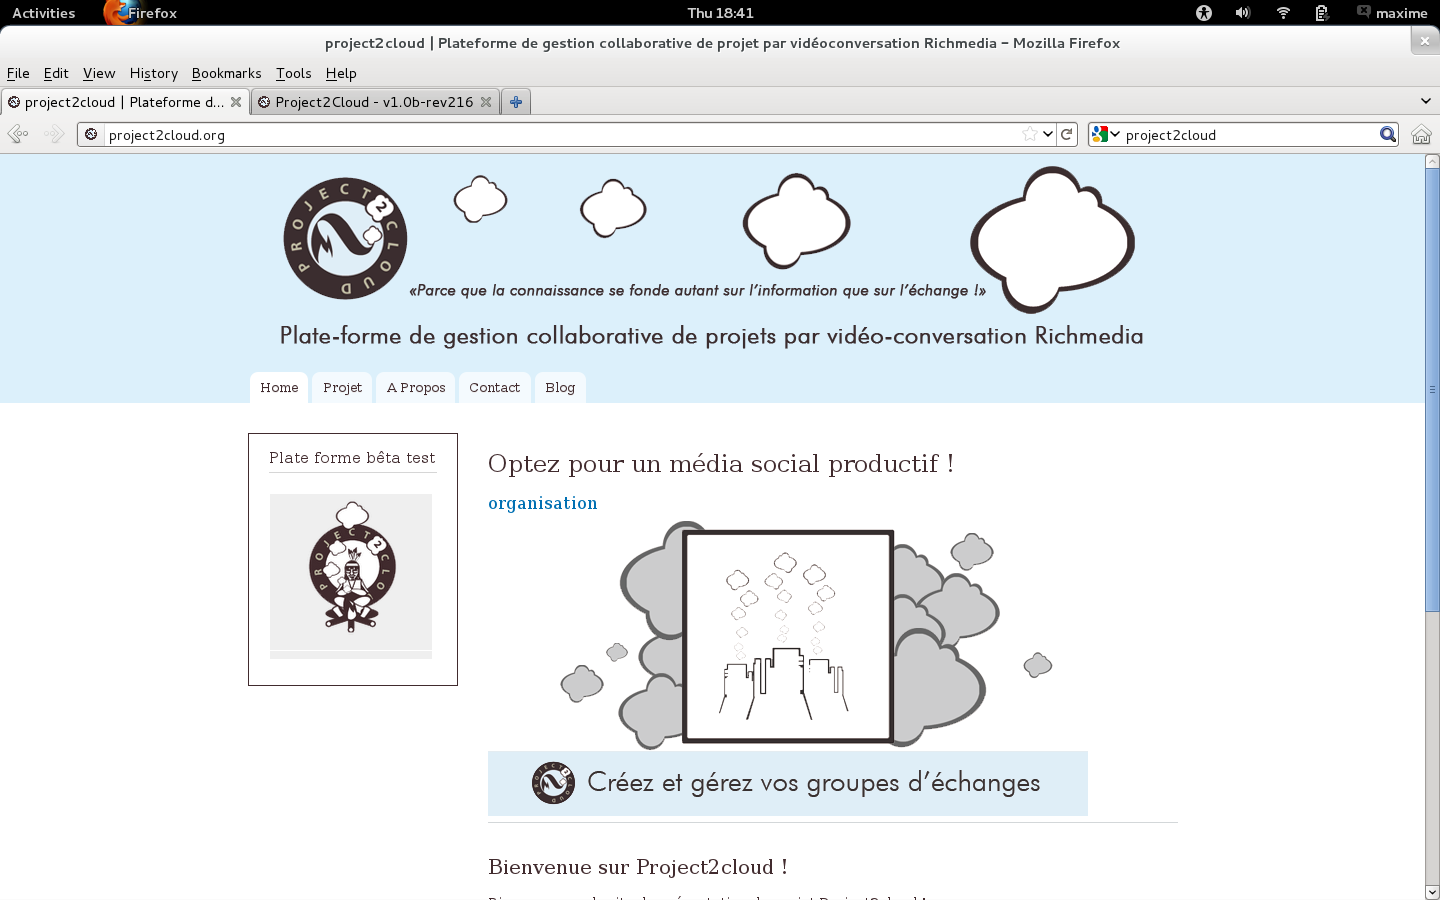
\includegraphics[width=350pt]{site.png}
					\caption{Site de présentation de l'application.}			
				\end{center}
			\end{figure}

	P2C (abréviation courante de Project2Cloud) est géré par trois informaticiens passionnés depuis maintenant 1 an. La plate-forme P2C est pour le moment en béta-test privé, c'est à dire qu'elle n'est pas encore accessible. Elle est actuellement testée par plusieurs industriels. Pour les besoins du projet, un accès nous a été donné à la version opérationnelle de la plate-forme. Cette version nous permet d'avoir une idée de l'application qui sera prochainement disponible. 

			\begin{figure}[H] 
				\begin{center}
					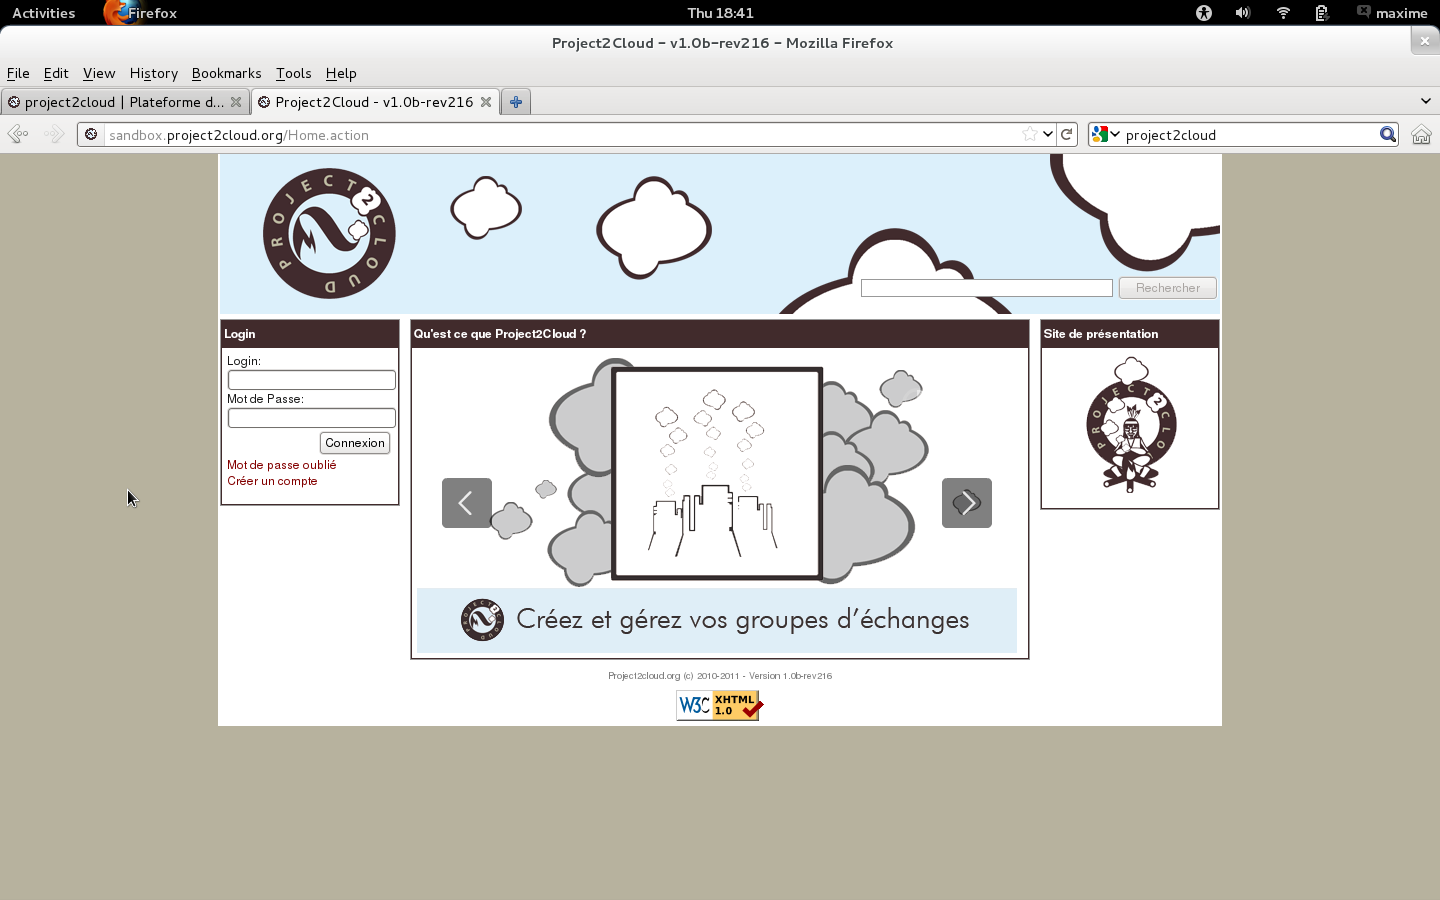
\includegraphics[width=350pt]{plateforme_d_essai}
					\caption{Plateforme Project2Cloud en béta-test.}			
				\end{center}
			\end{figure}
			
			\begin{figure}[H] 
				\begin{center}
					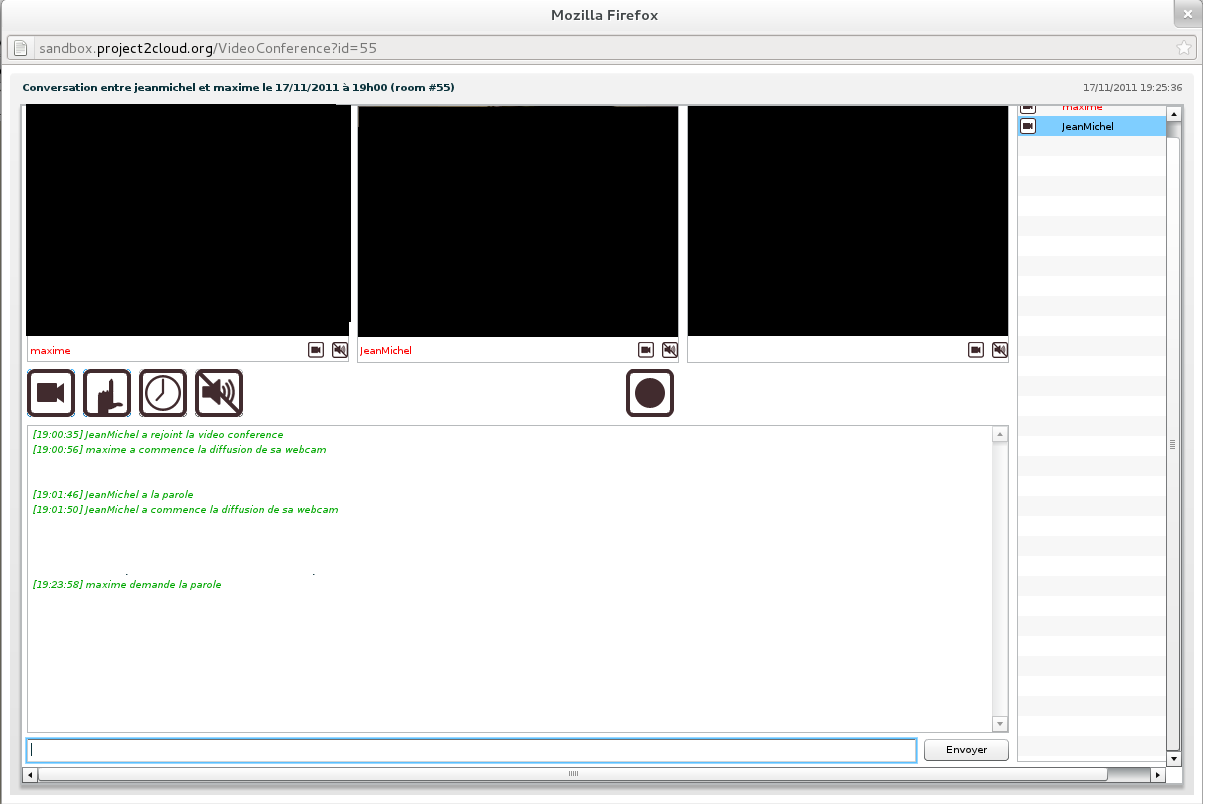
\includegraphics[width=350pt]{videoconf}
					\caption{Vidéo conférence avec Project2Cloud.}			
				\end{center}
			\end{figure}


	\section{Notre projet : Transcriptions audio vers texte pour des réunions enregistrées}
	Notre projet s'implantera directement dans la plate-forme P2C. Comme nous l'avons expliqué précédemment, P2C permettra aux utilisateurs de communiquer facilement grâce à un panel complet d'échanges vidéo, audio ou texte. Le but de notre projet est de faciliter l'indexation des conférences vidéos (c'est à dire de mieux séquencer temporellement les vidéos enregistrées). Pour cela, nous devrons ajouter une fonctionnalité supplémentaire : la transcription vocale des conversations. Concrètement, lors d'une conférence vidéo, les conversations des différents participants seront traduites en texte. Ce même texte sera enregistré sur un serveur. Le but est de permettre à un utilisateur de retrouver un mot ou un groupe de mot prononcé pendant une conférence, et de pouvoir visionner cette dernière à l'instant où le mot a été prononcé. On créé ainsi une "mémoire" des conférences, avec la possibilité de retrouver des informations très précises à des moments clés. 
	Notre projet est donc de convertir les conversations en texte, de les enregistrer, et de pouvoir indexer ces conversations à partir de mots clés. 

	\section{Analyse organisationnelle : dimension commerciale de notre projet}
	Notre projet vise donc à apporter une fonctionnalité supplémentaire à une plate-forme déjà existante. Cet aspect est intéressant, dans la mesure où des sites (ou des logiciels) proposant des conférences vidéos existent déjà (comme Skype par exemple). Project2Cloud propose de nouvelles options encore peu voire pas développée, dont notre projet de transcription vocale. On est donc en droit de se demander dans quelle mesure l'amélioration de la plateforme par notre projet peut-elle donner à l'entreprise l'opportunité d'étendre la distribution de son produit ?